%% The basic ESPResSo tutorial
%%
% Writer's guide lines:
% - provide background information and references
% - do not get lost in details but maintain a nice readability
% - describe every line of the script, that contains an ESPResSo
%   command (in future tutorial, only describe new ones) 
%
%%%%%%%%%%%%%%%%%%%%%%%%%%%%%%%%%%%%%%%%%%%%%%%%%%%%%%%%%%%%%%%%%
%%%%%%%%%%%%%%%%%%%%%%%%%%%%%%%%%%%%%%%%%%%%%%%%%%%%%%%%%%%%%%%%% 
% From the brainstorming:
%
% Preknowledge:
% 
% Basic MD(simple integrator,langevin thermostat, ---basic tcl
% basic potentials, basis tutorial 1
% 
% Basis Tutorial: written in Latex
% 
% <<every line of script code should be explained>>
% 
% 1) tcl basic setting up a system
% MD, soft sphere and Lennard-Jones Fluid (argon system), 
% Units
% 
% online visualization (pdb output)
% rdf, pressure,energy,
% 
% online analysis function
% savin, readin writeout, offline analysis, statistics
% 
% Structure:
% Part1:
% 1) Prerequisits (what you should know beforehand: basic tcl knowledge,
% Here you can find more info: Allen, Tildesley: Frenkel smit,
% Rappaport, tcl tutorial,
% 
% 2) Physics of the systems (argon, soft sphere system)
% 
% 3) Algorithms (verlocity verlet, Langevin, Potentials, LJ)
% 3b) about units
% 
% Part2 
% 1) simulation script in all detail, line by line
% Initialize
% Visualize
% Simulate (with online analysis, saves for later off-line analysis,
% (Savelize (save our lives ))
% 
% 2) a new script for later
% analysis, and other helper ideas
% 
% Things to remember and take care of:
% Use the same names for variables
% 
% ====================================================================
% General Tutorial: (the next tutorials: pe_solution, cell model of one
% charged colloid, LB, ferrofluid)
% 

% basiert auf KOMA-Script scrbook-Klasse
\documentclass[11pt,a4paper,% BCOR8mm,
	       %twoside, onecolumn, openright, cleardoubleempty, %
	       %parindent,
headnosepline, footnosepline, notitlepage, %
	       %onelinecaption,
bigheadings, % bibtotoc, %tocindent, listsindent, %
	       %chapterprefix, noappendixprefix,
	       %tablecaptionbelow,
	       %pointlessnumbers, % macht Probleme (Anhang ohne Punkt, aber sonst Kapitel mit Punkt
	       % abstractoff, fleqn, leqno,
	       % openbib, origlongtable,
final]{scrartcl}

% Satzspiegel 

% wenn keine KOMA-Klasse verwendet wird, kann so der Satzspiegel
% berechnet werden
%\usepackage[DIV15,BCOR12mm,pagesize]{typearea}

% Hier knnen Seitenhoehe und -breite individuell angepasst werden
%\areaset[BCOR]{Breite}{Hohe}
% oder 
%\usepackage[a4paper,body={15.6cm,23cm},left=3cm]{geometry}

% ============================================================================

%% Grafikpakete
% Fr einfache Einbingung von Grafiken
\usepackage{graphicx}%
\usepackage{framed, color}

% Wenn man direkt mit dem pdflatex eine PDF-Datei erzeugt, sollten diese beiden
% Pakete eingebunden werden (Hyperlinks, bessere Bildschirmschriftarten usw.)
\usepackage{color}
\definecolor{mylinkcolor}{rgb}{0.5812,0.0665,0.0659} % IndianRed 
\definecolor{mycitecolor}{rgb}{0.075,0.31,0.0431} % MossGreen 
\definecolor{myurlcolor}{rgb}{0.0118,0.098,0.7412} % DarkBlue
\usepackage[pdftex,bookmarks]{hyperref}

% Druckversion
% f�r reine pdf-Dateien noch Option colorlinks hinzufgen, um Links farbig zumachen
% \usepackage[pdftex,bookmarks,bookmarksopen,citecolor={mycitecolor},%
%  linkcolor={mylinkcolor},urlcolor={myurlcolor},breaklinks=true,%
%  hypertexnames=false,hyperindex=true,encap,colorlinks]{hyperref} %

%  	\hypersetup{
%     pdftitle = {},
%     pdfauthor = {Kai Grass},
%     pdfsubject = {},
%     pdfkeywords = {},
%     pdfcreator = {},%
%     pdfproducer = {},
% 	}%

\usepackage{ae,aecompl}

% ============================================================================

%% Sprachliche Pakete
\usepackage[english]{babel}
% Neue Deutsche Rechtschreibung
%\usepackage[ngerman]{babel}
%\usepackage{ngerman} 

% Paket zur einfacheren Eingabe deutscher Umlaute
%\usepackage[applemac]{inputenc} %Mac
%\usepackage[latin1]{inputenc}   %UNIX/LINUX
% \usepackage[ansinew]{inputenc}  % Windows
\usepackage[T1]{fontenc}

% ============================================================================

% Literaturverzeichnis
\usepackage[square,numbers,sort&compress]{natbib}
%\usepackage{bibmods}
%\bibpunct{(}{)}{,}{a}{}{,}
%\bibpunct{(}{)}{,}{a}{,}{;}
\setlength{\bibsep}{1ex}

% ============================================================================

% Stichwortverzeichnis
% \usepackage{makeidx}
% \makeindex

% ============================================================================

% Deutsche Zahlenkonvention (1 (Komma) 0 statt 1 (Punkt) 0)
% \usepackage{ziffer}

%% Schriftarten
\usepackage{times} % times is used to avoid bitmap fonts in PDF

%% Mathematische Packages
% Dieses Pakete definiert viele ntzliche mathematische Befehele und
% Die Option "intlimits" bewirkt, dass beim Integral die Grenzenangaben oben
% und unten erscheinen und nicht seitlich.
\usepackage[intlimits]{amsmath}
\usepackage{amsfonts}
\usepackage{amsthm}
\usepackage{mathrsfs}
\usepackage{stmaryrd}


% Diese Schriftarten ermglichen schne Mengensymbole fr natrliche Zahlen, usw.
% siehe Definition von \N, \Z usw. Dies ist Geschmackssache.
%\usepackage{bbm}
%\usepackage{dsfont}

% Subfigures
\usepackage{subfigure}

% Needed for Tabular-Umgebung
\usepackage{array}

% werden (sog. Schusterjungen und Hurenkinder vermeiden)
%\clubpenalty = 10000
%\widowpenalty = 10000

\sloppy

% Ein Paket um "kommutative Diagramme" zu erstellen. Fuer einfhrende Beispiele
% siehe xymanual.ps und xyreference.ps
%\usepackage[all]{xy}

%%%%%%%%%%%%%%%%%%% Shortcuts %%%%%%%%%%%%%%%%%%%%%%%%%%%%%%%%%%%%%%%%%%%%
%\newcommand{\N}{\mathbbm{N}}	% Natuerliche Zahlen
%\newcommand{\Z}{\mathbbm{Z}}	% Ganze Zahlen
%\newcommand{\Q}{\mathbbm{Q}}	% Rationale Zahlen
%\newcommand{\R}{\mathbbm{R}}	% Reelle Zahlen
%\newcommand{\C}{\mathbbm{C}}	% Komplexe Zahlen
%\newcommand{\one}{\mathbbm{1}}	% Einheits Eins
%
%\newcommand{\toinf}{\to\infty}				% --> oo
%\newcommand{\tozero}{\to 0}				% --> 0
%\newcommand{\ontop}[2]{\genfrac{}{}{0pt}{}{#1}{#2}}	% Aufeinander
%\newcommand{\abs}[1]{\left|#1\right|}
%\newcommand{\argmax}{\mathop{\rm arg\,max}}

% Ein Befehl, um Abbildungen einfach einheitlich zu gestalten
% Bsp: \abb{f}{\R}{\R}{x}{x^2}

%\newcommand{\abb}[5]{%
%\setlength{\arraycolsep}{0.4ex}%
%\begin{array}{rcccc}%
%#1 &:\,& #2 & \,\,\longrightarrow\,\, & #3 \\[0.5ex]%
%     & & #4 & \longmapsto & #5%
%\end{array}%
%}

%%%%%%%%%%%%%%%%%%% Theorem definitions %%%%%%%%%%%%%%%%%%%%%%%%%%%%%%%%%%
%\theoremstyle{plain}
%\newtheorem{theorem}{Theorem}[chapter]
%\newtheorem{proposition}[theorem]{Proposition}
%\newtheorem{lemma}[theorem]{Lemma}
%\newtheorem{satz}[theorem]{Satz}
%\newtheorem{korollar}[theorem]{Korollar}
%
%\theoremstyle{definition}
%\newtheorem{definition}{Definition}[chapter]
%\newtheorem{beispiel}[theorem]{Beispiel}
%\newtheorem{bemerkung}[theorem]{Bemerkung}
%
%%%%%%%%%%%%%%%%%%%%%%%%%%%%%%%%%%%%%%%%%%%%%%%%%%%%%%%%%%%%%%%%%%%%%%%%%%

% ============================================================================
% \renewcommand*{\partpagestyle}{empty}
% \renewcommand*{\partformat}{\partname~\thepart:}
%\usepackage{fancyhdr}
%%\pagestyle{headings}
%\pagestyle{fancyplain}
%%\addtolength{\headwidth}{\marginparsep}
%%\addtolength{\headwidth}{\marginparwidth}
%\renewcommand{\chaptermark}[1]{\markboth{#1}{}}
%\renewcommand{\sectionmark}[1]{\markright{\thesection\ #1}}
%%\lhead[\fancyplain{}{\bfseries\thepage}]{\fancyplain{}{\bfseries\rightmark}}
%\lhead[\fancyplain{}{\thepage}]{\fancyplain{}{\rightmark}}
%%\rhead[\fancyplain{}{\bfseries\leftmark}]{\fancyplain{}{\bfseries\thepage}}
%\rhead[\fancyplain{}{\leftmark}]{\fancyplain{}{\thepage}}
%%\chead{}
%%\rhead{\thepage}
%%\lfoot{Schnellste Pfade in geometrischen Netzwerken}
%\cfoot{}
%%\rfoot{}
%%\setlength{\headrulewidth}{0.4pt}
%%\setlength{\footrulewidth}{0.4pt}

%\usepackage[automark]{scrpage2}
%\pagestyle{scrheadings}
%\automark[section){chapter}
%\lehead[scrplain-links-gerade]{scrheadings-links-gerade}
%\cehead[scrplain-mittig-gerade]{scrheadings-mittig-gerade}
%\rehead[scrplain-rechts-gerade]{scrheadings-rechts-gerade}
%\lefoot[scrplain-links-gerade]{scrheadings-links-gerade}
%\cefoot[scrplain-mittig-gerade]{scrheadings-mittig-gerade}
%\refoot[scrplain-rechts-gerade]{scrheadings-rechts-gerade}
%\lohead[scrplain-links-ungerade]{scrheadings-links-ungerade}
%\cohead[scrplain-mittig-ungerade]{scrheadings-mittig-ungerade}
%\rohead[scrplain-rechts-ungerade]{scrheadings-rechts-ungerade}
%\lofoot[scrplain-links-ungerade]{scrheadings-links-ungerade}
%\cofoot[scrplain-mittig-ungerade]{scrheadings-mittig-ungerade}
%\rofoot[scrplain-rechts-ungerade]{scrheadings-rechts-ungerade}
%\ihead[scrplain-innen]{scrheadings-innen}
%\chead[scrplain-zentriert]{scrheadings-zentriert}
%\ifoot[scrplain-innen]{scrheadings-innen}
%\cfoot[scrplain-zentriert]{scrheadings-zentriert}
% Markierungen: \leftmark, \rightmark, \pagemark \headmark
% \manualmark \automark

% ============================================================================  

%%%%%%%%%%%%%%%%%%%%%%%%%%%%%%%%%%%%%%%%%%%%%%%%%%%%%%%%%%%%%%%%%%%%%%%%%%
\setcounter{secnumdepth}{2}
\setcounter{tocdepth}{1}
%%%%%%%%%%%%%%%%%%%%%%%%%%%%%%%%%%%%%%%%%%%%%%%%%%%%%%%%%%%%%%%%%%%%%%%%%%

%% Schriftsatz in KOMA
%\setkomafont{Element}{Befehle}
%\addtokomafont{Element}{Befehle}
%\usekomafont{Element}

%\includeonly{kapitel/sinterkeramiken, kapitel/statisch, kapitel/dynamisch, kapitel/ergebnisse, kapitel/abbildungen,
% kapitel/literatur}
%\includeonly{kapitel/titelseite2}
% ============================================================================

\usepackage{verbatim}
\usepackage[usenames,dvipsnames]{xcolor}

% The ESPResSo Logo
% how to define it such that there is a space afterwards if needed
% but not, when there is a point afterwards ????
\newcommand{\ES}{\textbf{ESPResSo}}

% How to diplay ESPResSo commands in flowing text. Larger code segments
% should be put inside boxes.
\newcommand{\EScmd}[1]{\texttt{\textbf{#1}}}

% The code block
%\newcommand{\EScode}[1]{ \parbox{0.95\textwidth}{\texttt{#1}}}

\definecolor{codebg}{rgb}{0.95,0.95,0.95}
\definecolor{codeframe}{gray}{0.5}
\definecolor{codeshadow}{gray}{0.7}
\definecolor{codenumber}{rgb}{0.58,0,0.82}
\definecolor{pblau}{rgb}{0.09375,0.19921875,0.4296875}

\usepackage{listings}
\lstset{
  basicstyle=\ttfamily,
	keywordstyle=\bfseries\ttfamily\color[rgb]{0.65,0.16,0.18},
	identifierstyle=\ttfamily\color{black},
	commentstyle=\color{pblau},
	stringstyle=\ttfamily\color[rgb]{0.627,0.126,0.941},
	showstringspaces=false,
	tabsize=2,
	breaklines=true,
	prebreak = \raisebox{0ex}[0ex][0ex]{\ensuremath{\hookleftarrow}},
	breakatwhitespace=false,
	numberstyle=\footnotesize \normalfont \sffamily,
	numbers=left,
	stepnumber=1,
	numbersep=1.5em,
  xleftmargin=2.7em,
  framexleftmargin=2.7em,
	aboveskip={1\baselineskip},
	belowskip={1\baselineskip},
  columns=fixed,
  upquote=true,
  extendedchars=true,
  frame=shadowbox,
  rulesepcolor=\color{codeshadow},
  rulecolor=\color{codeframe},
  backgroundcolor=\color{codebg},
  mathescape=false,
  language=tcl
}
%\lstset{numbers=left, numberstyle=\tiny, numbersep=5pt, showspaces=false, showstringspaces=false,postbreak=\space, breakindent=5pt, breaklines}
%\lstset{basicstyle=\ttfamily,keywordstyle=\color{blue}\bfseries,emphstyle=\color{green}, commentstyle=\color{red}\itshape,columns=fullflexible }
\lstset{keywordsprefix=setmd}
\lstset{keywords=[6]{thermostat,part,inter,integrate,rescale_velocities,code_info,save_sim,writepdb,analyze,uwerr, lbnode, lb_boundary, lbfluid, constraint,electrokinetics}}

\newcommand{\todo}[1]{{\color{BrickRed}\textbf{#1}}}


\newtheorem{task}{Task}

\usepackage{amssymb}
\usepackage[english]{babel}
\usepackage{bm}
\usepackage{graphicx}
\usepackage[utf8]{inputenc}
\usepackage{mathtools}
\usepackage[expansion=true,protrusion=true]{microtype}
%\usepackage{color}
\usepackage{textcomp}
\usepackage[usenames,dvipsnames]{xcolor}
\usepackage{cleveref}

\DeclareMathOperator\arctanh{arctanh}
\newcommand{\bad}[1]{{\color{blue} #1}}
\newcommand{\U}[1]{\,\mathrm{#1}}
\newcommand{\E}[1]{\times 10^{#1}}
\newcommand{\Z}{\mathbb{Z}}
\newcommand{\threevec}[3]{\begin{pmatrix} #1 \\ #2 \\ #3 \end{pmatrix}}
\newcommand{\lb}{l_\mathrm{B}}
\newcommand{\lD}{\lambda_\mathrm{D}}
\newcommand{\kT}{k_{B}T}
\newcommand{\tens}[1]{\overline{\bm{#1}}}
\let\vec\bm
\newcommand{\etal}{et~al.}
\newcommand{\ie}{i.e.,~}
\newcommand{\eg}{e.g.,~}
\newcommand{\joost}[1]{{\color{Plum}\uppercase{\textbf{#1}}}}
\newcommand{\georg}[1]{{\color{BrickRed}\textbf{#1}}}

\begin{document}
\renewcommand{\d}{\mathrm d}
\subject{ESPResSo Tutorial}
\title{The GPU Electrokinetics method in \ES{}: 
Electroosmotic Flow
} %\author{ Georg Rempfer \thanks{\ttfamily georg@icp.uni-stuttgart.de}}
\date{\today}
\publishers{Institute for Computational Physics, University of Stuttgart}
\maketitle 
\begin{center}
  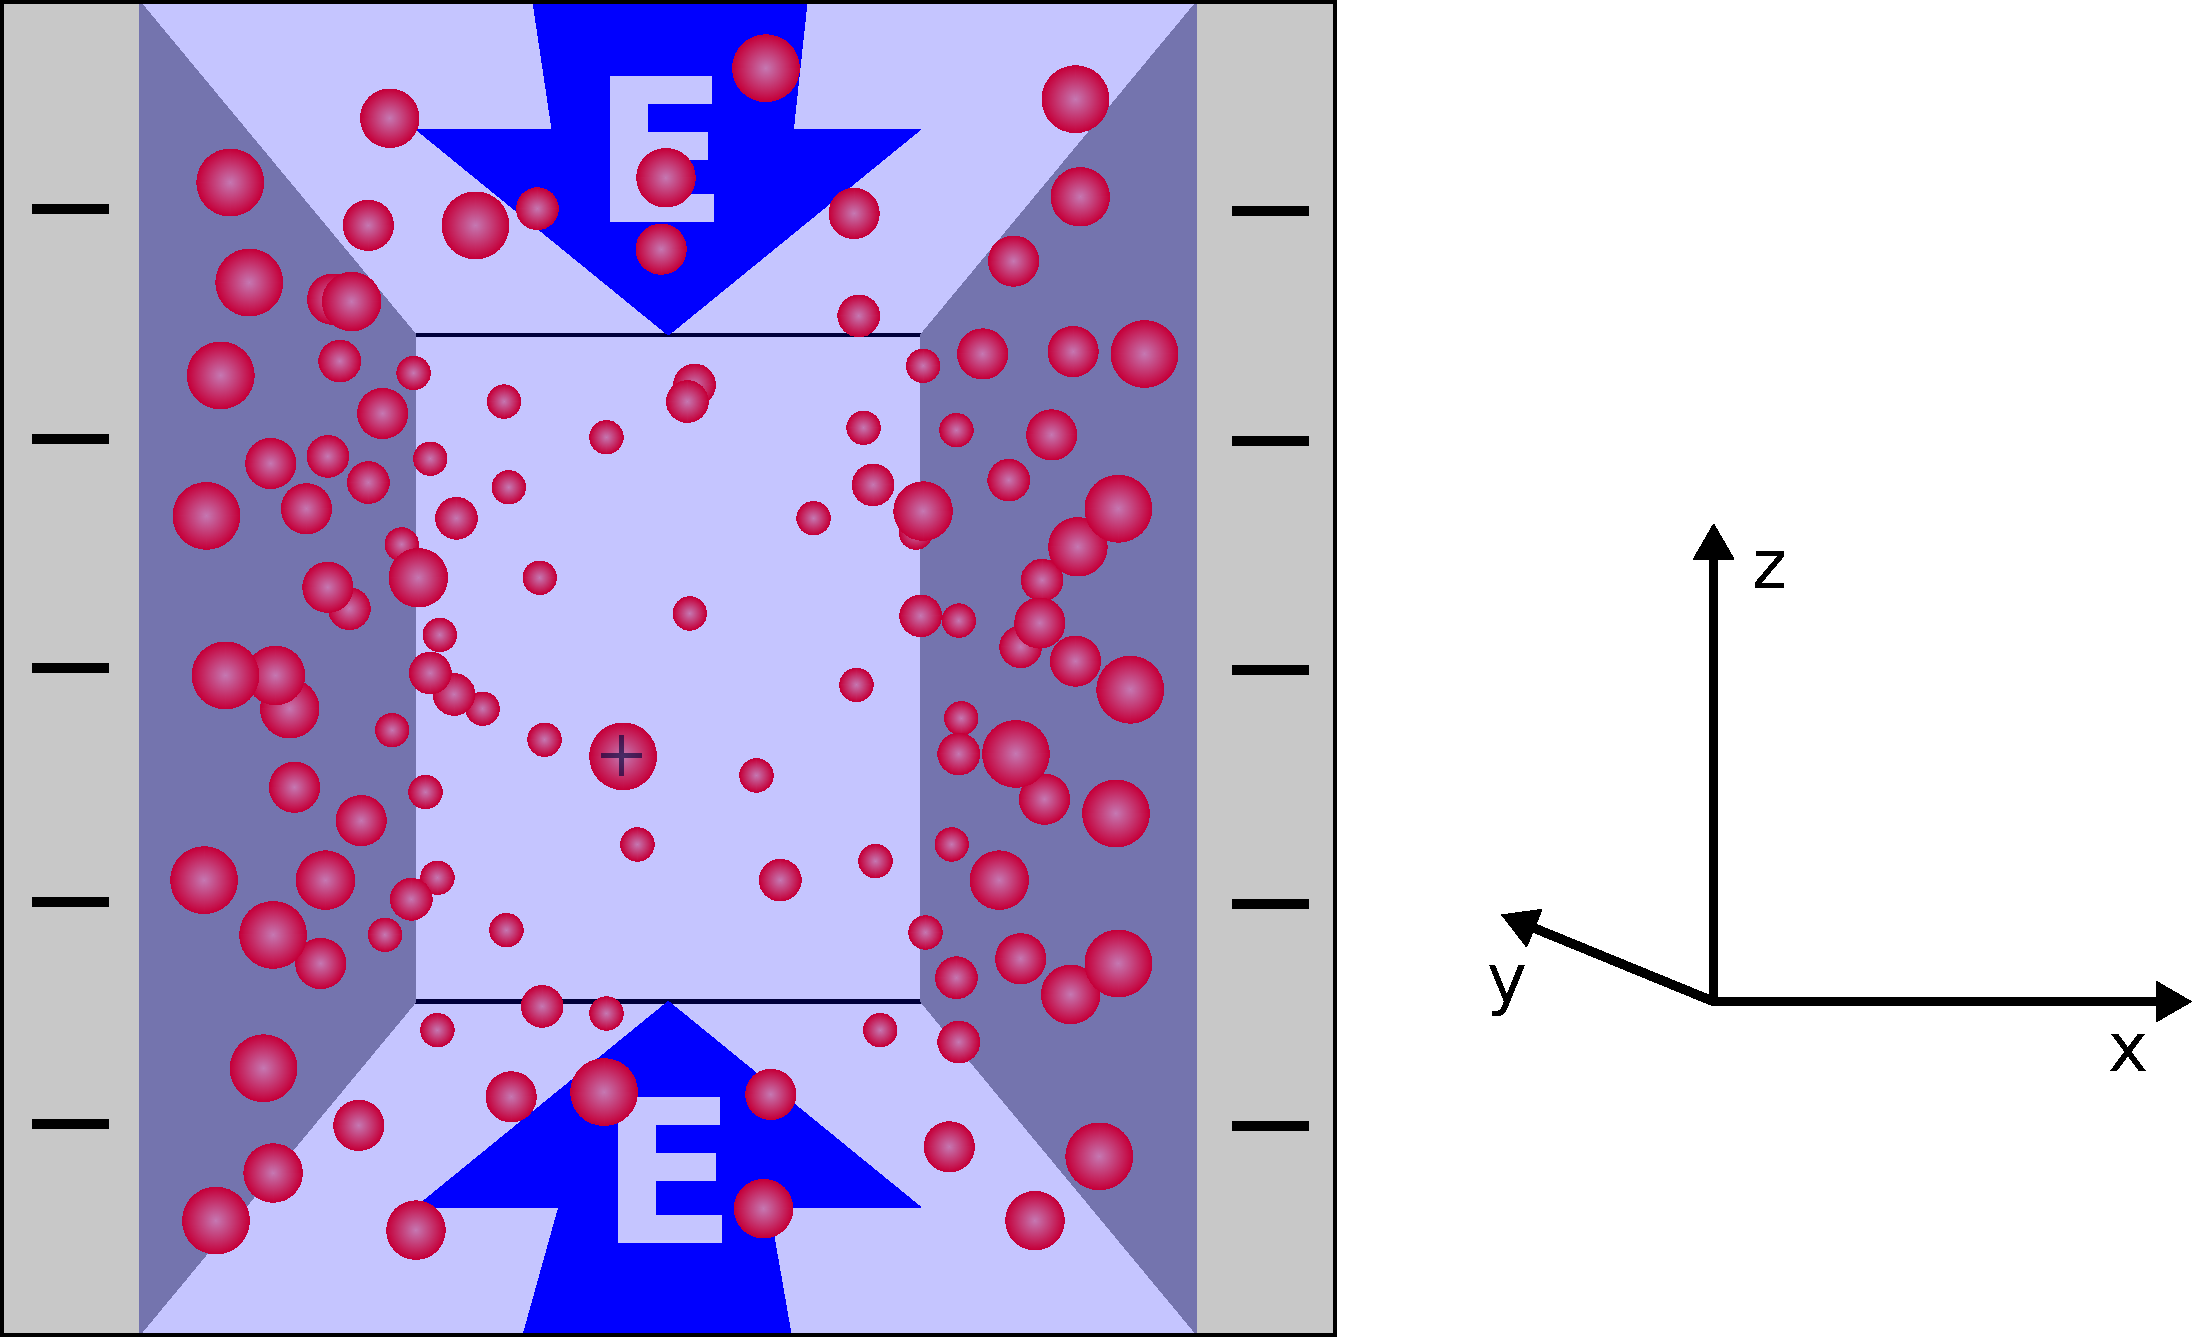
\includegraphics[width=0.7\columnwidth]{figures/schlitzpore_3d.pdf}
\end{center}
\pagebreak
\definecolor{mygray}{gray}{.75}
%\begin{center}
%  \colorbox{mygray}{ 
%\begin{minipage}[h]{13cm}
%  {\bf \large Before you start:}\\
%  With this tutorial you can get started using the Electrokinetics method
%  for scientific applications. We give a brief introduction about the theory
%  and how to use it \ES{}. 
%  We have selected one sample problem for which an analytic solution exists.
%\end{minipage}
%}
%\end{center}

 \tableofcontents
 \pagebreak
  
\section{Introduction}

%\floatingBox{5}{4cm}{Mein Text der in der Box abgebildet werden soll. Mal schauen wie das klappt.} 

In recent years the lattice-Boltzmann method (LBM) has proven itself to be a viable way to introduce hydrodynamic interactions into coarse-grained MD simulations with moderate computational cost. The success of the GPU LBM implementation in \ES{} and similar developments in other software packages created demand for further developments in this area. \ES{} features two such algorithms, namely ELECTROHYDRODYNAMICS, and ELECTROKINETICS (EK). Both of these make use of the LBM and extend it to coarse-grain not only the solvent molecules but also ionic solutes. ELECTROHYDRODYNAMICS does so using a slip layer coupling for charged particles valid in the thin Debye layer (large salt concentration) limit, while EK explicitly treats the ionic solutes in a continuum fashion and is valid for a wide range of salt concentrations.

\subsection*{Tutorial Outline}

To make our first steps using ELECTROKINETICS we will work on one of the few systems for which analytic solutions for the electrokinetic equations exist -- the slip pore geometry with a counterion-only electrolyte. The same slit pore system is also treated in the LBM tutorial, but there, the ionic species were modeled as explicit particles. For this system, the two approaches lead to exactly the same results~\cite{rempfer10a}. Differences are only becoming significant for multivalent ions, very high salt concentrations, and very high surface charges.

This tutorial is divided into three sections. The first section~\ref{sec:theory} introduces the electrokinetic equations and the analytical solution for the slit pore system, while the second section~\ref{sec:simulation} deals exclusively with the simulation, its setup, and the results.

If you already know about simple diffusion-migration-advection equations, continuum electrostatics, and Navier-Stokes, then you can skip the first section.

\pagebreak

%\section{\label{sec:vmd}VMD}

This tutorial currently only covers visualization using Paraview. Refer to the User's Guide for information on how to visualize \ES{} simulations with VMD.

\pagebreak

\section{\label{sec:paraview}Paraview}

For this part of the tutorial we are going to use Paraview, an easy to use, open source visualization program for scientific data. You should find a preinstalled version on the CIP pool computers, which you can execute with the command
%
\begin{center}
\texttt{paraview}
\end{center}
%
If you want to use it on other computers, it is part of most Linux distributions' repositories or you can get a copy at \href{http://www.paraview.org/}{http://www.paraview.org/}.

You can output the LB velocity field and the boundary geometry from \ES{} in a Paraview compatible format with the following commands
%
\begin{itemize}
\item \texttt{lbfluid print vtk boundary \textit{filename}}
\item \texttt{lbfluid print vtk velocity \textit{filename}}
\end{itemize}
%
while the particle coordinates can be output using
\begin{itemize}
\item \texttt{writevtk \textit{filename} [\textit{particle-type}]}
\end{itemize}
%
If no particle type id is given, all particle coordinates are written.

Filenames should always carry the suffix \texttt{.vtk}, so that Paraview automatically selects the correct reader upon opening. If you want to create a time series (video), you should name your files \texttt{filename\_CTR.vtk} with CTR a number incremented for every frame. You can then load all these files at one with Paraview and use the video controls to step through time.

Paraview is a very flexible visualization program. You can use the GUI to create very specific visualizations for your data. Visualization methods and data post processing algorithms are contained in so-called \textit{filters}. Filters can be chained and filter chains form a \textit{pipeline} which can be manipulated using the \textit{pipeline-browser}. For a start, it will be sufficient to know about the 7 Paraview controls shown in Figure~\ref{fig:paraview}.
%
\begin{figure}[htp]
\begin{center}
  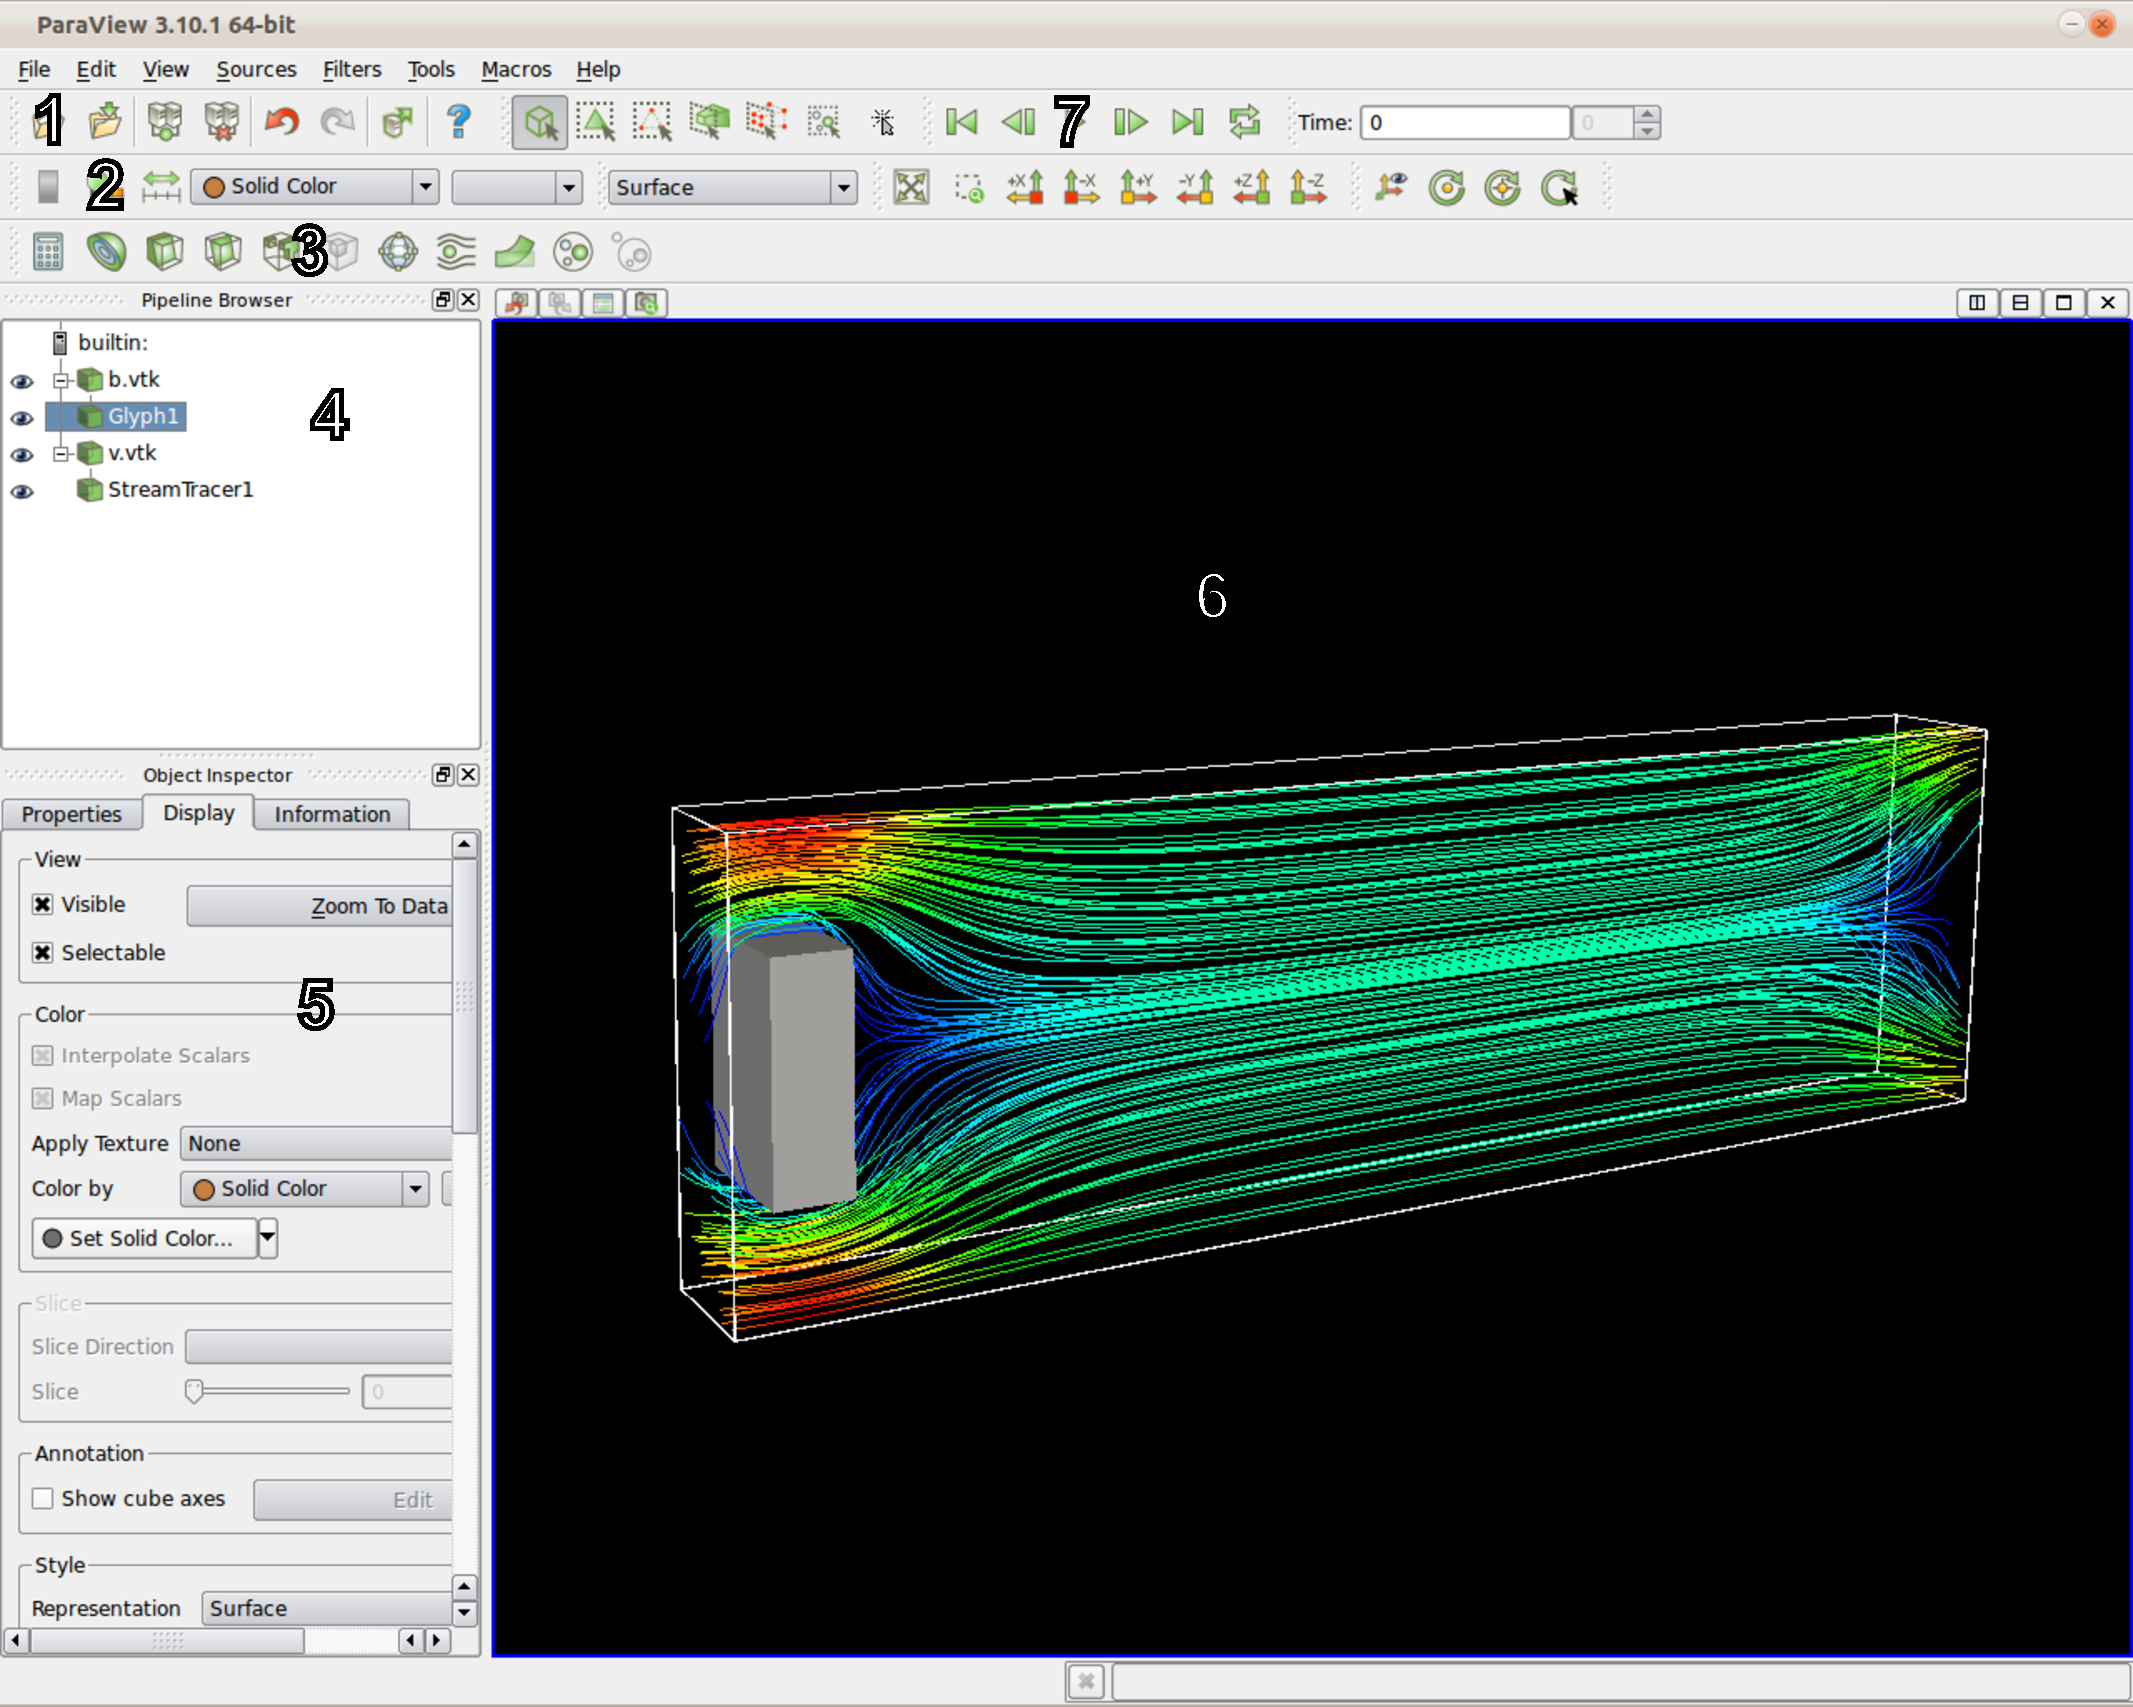
\includegraphics[width=1.0\textwidth]{figures/paraview.pdf}
  \caption{Paraview with a sample visualization and the most important controls.}
  \label{fig:paraview}
\end{center}
\end{figure}
%
\begin{enumerate}
\item Load data files into the pipeline for visualization
\item Adjust color settings of the filter selected in the pipeline browser
\item Add one of the most used filters to the element selected in the pipeline browser
\item The pipeline browser -- shows loaded data files and filter applied to them for visualization
\item Configuration panel for the filter chosen in the pipeline browser
\item The preview panel -- you can rotate, zoom and move this with the mouse
\item Controls for videos
\end{enumerate}
%
For a start it makes sense to use a \textit{Glyph} filter to visualize particle positions and a \textit{Slice}, \textit{Streamline}, or \textit{Glyph} filter for LB velocity fields. With a little exploration, these controls should be self explanatory. If you need help, don't hesitate to consult your tutor, the Paraview help (F1) or the Paraview online documentation at \href{http://www.paraview.org}{http://www.paraview.org}.

\pagebreak

\bibliographystyle{unsrt}
\bibliography{refs}
\end{document}

